\section{Characterizing Knowledge Markets}
In this section we characterize the knowledge markets in Stack Exchange---explaining the best-fit models and their foundations (Section 7.1), revealing two key distributions that control the markets (Section 7.2), and uncovering the stable core that maintains market equilibrium (Section 7.3).

\subsection{Model Interpretation} 
First, we explain the best-fit models found in Section 6.1. We observe that content generation in Stack Exchange markets are best modeled through the combination of power basis and interactive essential interaction. In addition, we found that the best-fit exponents ($\lambda$ parameter in basis $g(x) = ax^\lambda$, where $x$ is a factor) of these models lie between 0 and 1 (inclusive), for all factors of all content types, for all Stack Exchange. 

A model that uses power basis (where exponents lie between 0 and 1) and interactive essential interaction is known as the Cobb-Douglas production function~\cite{wiki}. In its most standard form for production of a single output $z$ with two inputs $x_1$ and $x_2$, the function is: 
$$z = ax_1^{\lambda_1}x_2^{\lambda_2}.$$
Here, coefficient $a$ represents the \emph{total factor productivity}---the portion of output not explained by the amount of inputs used in production~\cite{wiki}. As such, its level is determined by how efficiently the inputs are utilized in production. The exponents $\lambda$s represent the \emph{output elasticity} of the inputs---the percentage change in output that results from the percentage change in a particular input~\cite{wiki}. 

The Cobb-Douglas function provides intuitive explanation for content generation in Stack Exchange markets. In particular, the explanation stands on three phenomena or principles: constant elasticity, diminishing returns, and returns to scale.

\textbf{Constant Elasticity.} In Stack Exchange markets, factors such as user participation and content dependency have \emph{constant elasticity}---percentage increase in any of these inputs will have constant percentage increase in output~\cite{wiki}, as claimed by the corresponding exponents in the model. For example, in \texttt{academia} ($N_A = 6.93N_q^{0.18}U_a^{0.65}$), 1\% increase in number of answerers ($U_a$) leads to 0.65\% increase in number of answers ($N_a$). 

\textbf{Diminishing Returns.} For a particular factor, when the exponent is less than 1, we observe \emph{diminishing returns}---decrease in the marginal (incremental) output as an input is incrementally increased, while the other inputs are kept constant~\cite{wiki}. This \lq law of diminishing returns\rq\ has many interesting implications for the Stack Exchange markets, including the diminishing benefit of having a new participant in a market. For example, in \texttt{academia}, if the number of answerers is 100, then the marginal contribution of a new answerer is $c(101^{0.65} - 100^{0.65}) = 0.129c$, where $c$ is a constant; in contrast, if the number of answerers is 110, then the marginal contribution of a new answerer is $c(111^{0.65} - 110^{0.65}) = 0.125c$. Thus, for answer generation in \texttt{academia}, including a participant when the number of participants (system size) is 110 is likely to be less beneficial compared to including a participant when the system size is 100.

\textbf{Returns to scale.} The knowledge markets in Stack Exchange vary in terms of scale efficiency, as manifested by their \emph{returns to scale}---the increase in output resulting from a proportionate increase in all inputs~\cite{wiki}. If a market has high returns to scale, then greater efficiency is obtained as the market moves from small- to large-scale operations. For example, in \texttt{academia}, for answer generation, the returns to scale is $0.18+0.65=0.83<1$. The market becomes less efficient as answer generation is expanded, requiring more questions and answerers to increase the number of answers by same amount. 

\subsection{Two Key Distributions} 
Next, we discuss two key distributions that control content generation in knowledge markets, namely participant activity and subject POV (perspective). These two distributions induce the three phenomena reported in section 7.1. 

\textbf{Participant Activity.} The distribution of participant activities implicitly drives a market's return in terms of user participation, as manifested by the corresponding exponent. For example, in a hypothetical knowledge market where each answerer contributes equally, the answer generation model should be $N_a = AN_q^{\lambda_1}U_a^{1.0}$. In reality, the distribution of participant activities is a size dependent distribution controlled by the number of participants (system size). As the system size increases, most participants contribute to the head of the distribution (few activities), whereas very few join the tail (many activities). 

We systematically reveal the size dependent distribution for participant activities in three steps. First, we empirically fit power-law distribution to the activities of participants in a month, for each month, for each Stack Exchange. We follow the standard procedure to fit a power-law distribution. We observe that power-law well describe the monthly activity distributions. Second, we plot the exponents of power-law against the number of participants for all observed months in a Stack Exchange, for each Stack Exchange. We observe that for most Stack Exchange power-law exponent decreases as the system size increases. Third, we apply linear regression to reveal the relationship between power-law exponents and system size. We observe that in general power-law exponents are negatively correlated with system size. This negative correlation is strongly visible in big knowledge markets that have at least 500 monthly participants in each month.

\begin{figure}[hbt]
\vspace{-0.5\baselineskip}
\centering
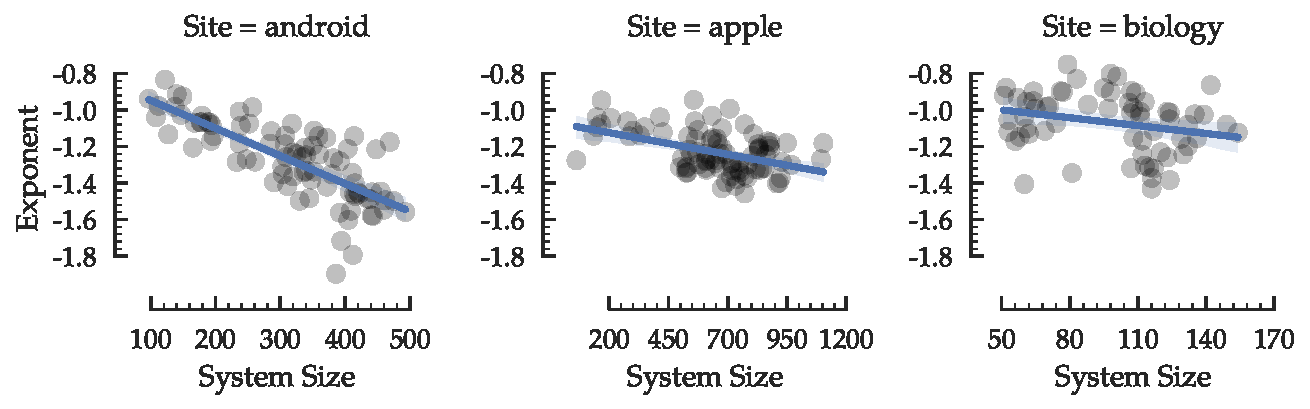
\includegraphics[scale=0.38]{Figures/Size_Dependent_Distribution.pdf}
\vspace{-2\baselineskip}
\caption{The visibility of size dependent distribution in \texttt{android} (strong), \texttt{apple} (moderate), and \texttt{biology} (weak). In most markets, the power-law exponent decreases with system size (similar to academia). In other markets, there exists a non-zero correlation between system size and power-law exponent.}
\vspace{-\baselineskip}
\label{fig:sdd}
\end{figure}

In Figure~\ref{fig:sdd} we present empirical evidence of size dependent distribution for answer generation in three markets: \texttt{android}, \texttt{apple}, and \texttt{biology}. We choose these examples to cover three possible visibility of size dependent distribution, as manifested by the correlation between 
power law exponent and system size---strong correlation ($|r^2|>0.5$), moderate correlation($0.3<|r^2|<0.5$), weak correlation ($|r^2|<0.3$).

\textbf{Subject POV.} The distribution of subject POV implicitly drives a market's return in terms of content dependency, as manifested by the corresponding exponent. Subject POV refers to the number of distinct perspectives on a particular content (primarily question) that imposes a conceptual limit to the number of dependent contents (answers). For example, an open-ended question such as \lq What's your favorite book?\rq\ has many possible answers, whereas a close-ended question such as \lq What's the solution for 3x+5 = 2?\rq\ has a single correct answer. In reality, most questions are neither completely open-ended nor completely closed; however, from an answerer's perspective, there's a diminishing utility in answering a question that already has an answer. This diminishing utility varies from question to question---questions asking for recommendations attract many answers, whereas questions seeking factual information attract few answers. 

\subsection{Uncovering the Stable Core} 
Now, we discuss about the core user community that assist maintaining the Cobb-Douglas models in a knowledge market. The Cobb-Douglas models indicate the presence of dynamic equilibria where the increase or decrease in user community does not affect the models. To this end, we assert that there is a stable user community in each knowledge markets who contribute a large fraction of contents; whereas the remaining users are unstable and contribute a small fraction. This is particularly applicable for high-threshold contents that require more effort, e.g, answers and comments. 

We reveal the presence of core user community by summarizing the age of users with different levels of contribution for all Stack Exchange. First, we categorize all users in all Stack Exchange into 10 categories based on their average number of contributions per month. Then, for each category, we compute average age of all users within the category. Next, we summarize the normalized age of users with same levels of contribution for all markets using letter value plots. This allows us to observe the global distribution of normalized age for users with varying levels of monthly contribution. We present these distributions in Figure~\ref{fig:age_vs_contribution}. We observe that there is a clear gap between the distribution of age of users for any two levels of contribution---users in 4th quartile (who contribute a lot) have highest normalized age, followed by 3rd and 2nd quartile. 

\begin{figure}[hbt]
\centering
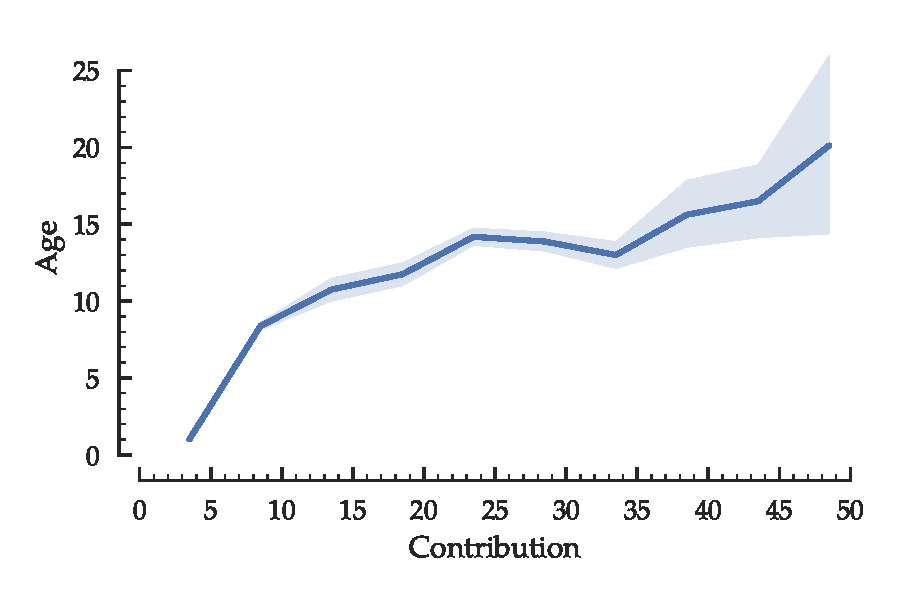
\includegraphics[scale=0.5]{Figures/Age_vs_Contribution.pdf}
\caption{The average age for users with varying levels of monthly contribution across all Stack Exchange. The users who contribute a lot to any market on a monthly basis, also contribute for many months as manifested by the average age.}
\label{fig:age_vs_contribution}
\end{figure}


